\subsection{Published-label legal component results}
Eleven of twelve checkpoint conditions have completed the four-task diagnostic; the Mistral 7B reference remains pending model-weight recovery. Table~\ref{tab:revision-legalbench} separates accuracy from class-balanced outcomes. The larger pretrained checkpoint differs in both model family and size; it provides a reference for component difficulty. The released seed and case contrasts include uncertainty, and probability metrics accompany each task.

\begin{table}[t]
\caption{Published-label LegalBench component diagnostics on 492 fixed cases. Entries are percent; adapted rows average five shared checkpoints, pretrained rows evaluate one checkpoint.}
\label{tab:revision-legalbench}
\centering
\small
\resizebox{\linewidth}{!}{%
\begin{tabular}{lrrrr}
\toprule
Task & Checkpoint & Accuracy & Macro F1 & Balanced accuracy \\
\midrule
Overruling & Qwen base & 49.2 & 43.8 & 51.5 \\
Overruling & FedAvg shared & 52.3 & 45.4 & 54.2 \\
Overruling & FLEN shared & 51.8 & 44.9 & 53.5 \\
UCC/common law & Qwen base & 57.4 & 36.5 & 50.0 \\
UCC/common law & FedAvg shared & 57.4 & 36.5 & 50.0 \\
UCC/common law & FLEN shared & 57.4 & 36.5 & 50.0 \\
Citation support & Qwen base & 53.7 & 47.9 & 53.7 \\
Citation support & FedAvg shared & 49.3 & 41.2 & 49.3 \\
Citation support & FLEN shared & 49.1 & 42.4 & 49.1 \\
Personal jurisdiction & Qwen base & 42.0 & 29.6 & 50.0 \\
Personal jurisdiction & FedAvg shared & 54.4 & 46.3 & 56.0 \\
Personal jurisdiction & FLEN shared & 55.2 & 46.4 & 55.2 \\
\bottomrule
\end{tabular}
}
\end{table}


Shared adaptation has task-dependent effects. FedAvg and FLEN reach 52.3\% and 51.8\% on overruling, compared with 49.2\% for the base checkpoint. On citation support, their means fall to 49.3\% and 49.1\% from 53.7\%. All three conditions produce the same UCC/common-law accuracy of 57.4\% with balanced accuracy 50.0\%, revealing a single-class solution. Personal-jurisdiction accuracy increases from 42.0\% to 54.4\% and 55.2\%, while balanced accuracy remains below 56\%. These outcomes identify limited component transfer and motivate expert authority annotation and independently verified citation retrieval.

\begin{figure}[t]
\centering
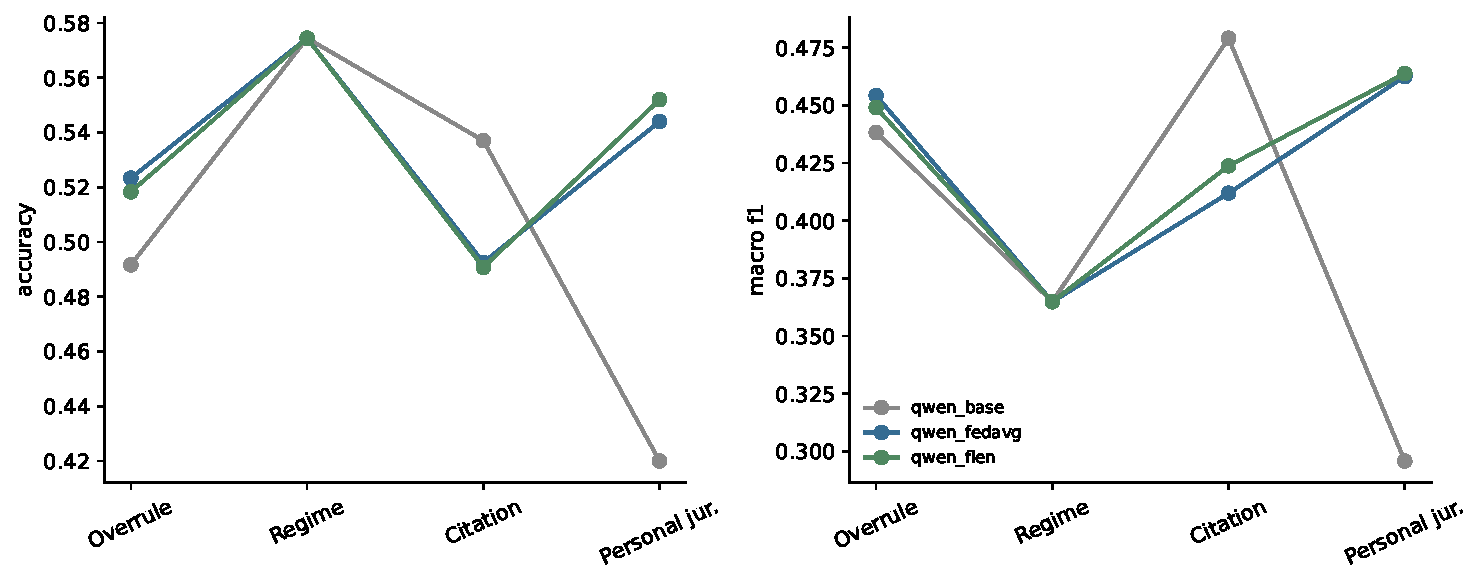
\includegraphics[width=\linewidth]{revision_legalbench.pdf}
\caption{Fixed-case component diagnostics; adapted values average five training seeds. Tasks retain their published label spaces.}
\label{fig:revision-legalbench}
\end{figure}
